\documentclass[12pt, a4paper]{article}
\usepackage[french]{babel}
\usepackage[T1]{fontenc}
\usepackage[utf8]{inputenc}
\usepackage{listings}
\usepackage{graphicx}
\usepackage{fancyhdr}
%\pagestyle{fancy}
\usepackage[a4paper,top=2cm,bottom=2cm,left=3cm,right=3cm,marginparwidth=1.75cm]{geometry}
\usepackage{xcolor}
\usepackage[french,vlined,lined,linesnumbered,boxed]{algorithm2e}
\usepackage{parskip}
\usepackage{hyperref}
\usepackage{amsmath}
\RequirePackage{float}

\usepackage{color}
\definecolor{lightgray}{rgb}{.9,.9,.9}
\definecolor{darkgray}{rgb}{.4,.4,.4}
\definecolor{purple}{rgb}{.96, .27, .57}
\lstdefinelanguage{JavaScript}{
  keywords={break, case, catch, continue, debugger, default, delete, do, else, false, finally, for, function, if, in, instanceof, new, null, return, switch, this, throw, true, try, typeof, var, void, while, with, class, export, throw, implements, import, this, boolean, number},
  morecomment=[l]{//},
  morecomment=[s]{/*}{*/},
  morestring=[b]',
  morestring=[b]",
  ndkeywords={T, Graph, List, Map, Grey, Blue, Red, Green, Rainbow},
  keywordstyle=\color{purple}\bfseries,
  ndkeywordstyle=\color{blue}\bfseries,
  identifierstyle=\color{black},
  commentstyle=\color{darkgray}\ttfamily,
  stringstyle=\color{red}\ttfamily,
  sensitive=true
}

\lstset{ 
  backgroundcolor=\color{white},   
  basicstyle=\footnotesize\ttfamily,        
  breakatwhitespace=false,         
  breaklines=true,                 
  captionpos=b,                    
  commentstyle=\color{mygreen},    
  firstnumber=1,                
  frame=single,	                
  keepspaces=true,                
  keywordstyle=\color{blue},       
  language=JavaScript,                 
  numbers=left,                    
  numbersep=5pt,                   
  numberstyle=\tiny\color{darkgray}, 
  rulecolor=\color{black},        
  showspaces=false,                
  showstringspaces=false,          
  showtabs=false,                  
  stepnumber=1,                   
  stringstyle=\color{mymauve},     
  tabsize=2,	                   
  title=\lstname            
}

\begin{document}

\begin{titlepage}
	\newgeometry{right=2.5cm, left=2.5cm, top=2.5cm, bottom=2.5cm}
	\begin{center}
		
		\vspace*{4cm}
		{ \Huge \bfseries Projet semestre 6} \\
		\vspace*{0.5cm}
		{ \Huge \bfseries Megalopolis}

		\vspace*{1cm}
		\textbf{Réalisé par :}\\
		\Large Romane Cavey\\
            \Large Gael Valade\\
            \Large Alexis Brandner\\
            \Large Faustine Lacroix\\
		
		\vspace*{3cm}

		\Large \textbf{Département Informatique}\\
		\Large \textbf{S6 - Année 2023/2024}\\
		
        \vspace{5cm}
		
		\begin{flushright}
		    
\includegraphics[width=6cm]{images/Enseirb.png}
        \end{flushright}1
		
	\end{center}
	\restoregeometry
\end{titlepage}

\newpage
\tableofcontents
\newpage

%%% Introduction :
\section{Introduction}
\label{sec:intro}

Le projet Megalopolis est un projet qui s'inspire fortement du jeu de société du même nom qu'il faut programmer en TypeScript par équipe de quatre.

\subsection{Rappel du sujet}
Il y n'a qu'un seul joueur, ce dernier pioche des tuiles contenues dans une pioche. Chaque tuile est composée de quatre quartiers et d'une route, c'est-à-dire d'un parc, d'une zone commerciale, d'une zone résidentielle, d'une zone industrielle et d'une route traversant les trois dernières zones. Le joueur peut poser deux tuiles côte à côte ou les superposer partiellement ou totalement tant qu'il y a au moins un quartier superposé. Le but du joueur est de maximiser ses points en fonction de 5 objectifs piochés en début de partie.

\subsection{Analyse du sujet}
Tout d'abord ce jeu repose sur des éléments de base tel que les quartiers, les routes, les tuiles et le plateau de jeu. La mise en place de ces éléments doit être comprise par tous les membres pour être manipulés sans difficultés. 

Dans un deuxième temps, le jeu nécessite la mise en place d'une pioche, d'objectifs et de la boucle de jeu pour pouvoir lancer des parties variées. Ensuite il faut implémenter un graphe pour les routes et un pour les quartiers. Enfin il faut calculer les scores pour avoir un jeu fonctionnel. Afin d'avoir des parties intéressantes, il faut trouver une bonne stratégie pour le joueur et si possible faire un affichage plaisant.

Nous avons essayé de suivre cette ligne directrice lors des séances de projet.

\subsection{Attendus}
Ce projet comportait une grande contrainte. En effet il était attendu que nous programmions ce projet de manière fonctionnelle et pure. Autrement dit, nous avons du mettre en pratique tout ce que nous avons appris lors du cours de PG104 avec le typage de données proposé par TypeScript, l'utilisation de types immutables tels que les listes et les dictionnaires de la librairie \texttt{Immutable.js}, l'utilisation de fonctions récursives et de fonction très utile comme \texttt{sort}, \texttt{reduce} et \texttt{map} et l'utilisation de Jest pour simplifier l'écriture des tests.



%%% Implémentation :
\input{parties/implémentation}


%%% Affichage :
\section{Affichage}

Dans ce projet, l'affichage est indispensable pour nous permettre d'avoir un appui visuel, certes les tests nous permettent de vérifier notre code, mais l'affichage visuel nous permet de mieux nous rendre compte de ce que nous faisons. Pour cela, nous avons deux manières d'afficher notre plateau, une manière primitive dans le terminal et une avec une interface web.

\subsection{Affichage primitif}

Dans un premier temps le but est d'afficher de manière simple, pour cela partant de l'implémentation vu en partie \ref{subsec:tile}. Pour cela nous utilisons des flèches "←↑" pour indiquer les entrées de route (ici "←↑" correspond à un type \texttt{Road} : \{$north$: true, $west$: true, $south$: false, $east$: false\}, 0 si il n'y a pas de route. Et pour les quartiers nous colorons le fond des flèches dans la couleur du quartier ce qui nous donne la tuile suivant en figure \ref{fig:tile_terminal}.


Ce premier affichage nous a permis de mieux avancer dans le projet mais il nous a fallu ensuite pouvoir voir le plateau décrit en partie \ref{subsec:board}. Comme celui-ci est représenté en \texttt{Quarter} il est facile de le représenter dans le terminale en trouvant l'ordonnée maximum et l'abscisse minimum puis d'afficher deux espaces si il n'y a pas de \texttt{Quarter} sinon afficher le \texttt{Quarter} et faire un retour a la ligne a chaque changement de ligne ce qui nous donne la figure \ref{fig:board_terminal}.

\begin{figure}[h]
    \centering
    \begin{minipage}{0.45\textwidth}
        \centering
        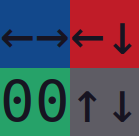
\includegraphics[width=0.5\linewidth]{images/Affichage/tile_termianl.png}
        \caption{Exemple d'affichage de tuile}
        \label{fig:tile_terminal}
    \end{minipage}\hfill
    \begin{minipage}{0.45\textwidth}
        \centering
        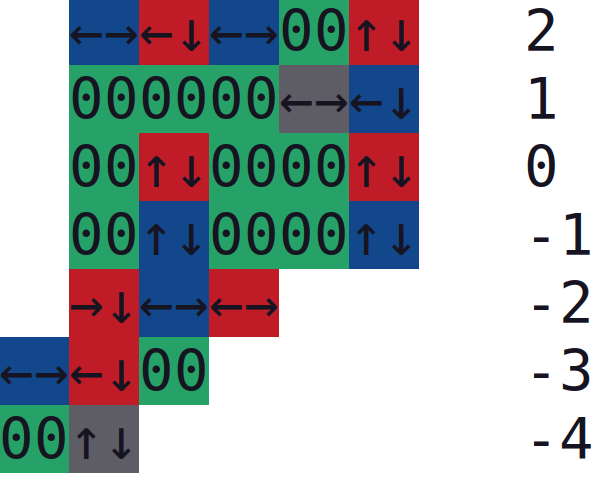
\includegraphics[width=0.5\linewidth]{images/Affichage/board_terminal.png}
        \caption{Exemple d'affichage du plateau}
        \label{fig:board_terminal}
    \end{minipage}
\end{figure}

\subsection{Affichage web}

Le projet proposait de créer une interface web permettant de visualiser des parties de Megalopolis. Cette interface, esthétiquement plus plaisante et interactive se fait à l'aide d'une page HTML, d'une feuille CSS et d'un script écrit en TypeScript permettant de lier notre page HTML au code réalisé pour le reste du projet.

\subsubsection{Interface graphique — HTML}

L'interface graphique se sépare en deux grands morceaux~: le plateau de jeu et le panneau de contrôle (voir Figure~\ref{fig:web_gui}).

\begin{figure}[h]
    \centering
    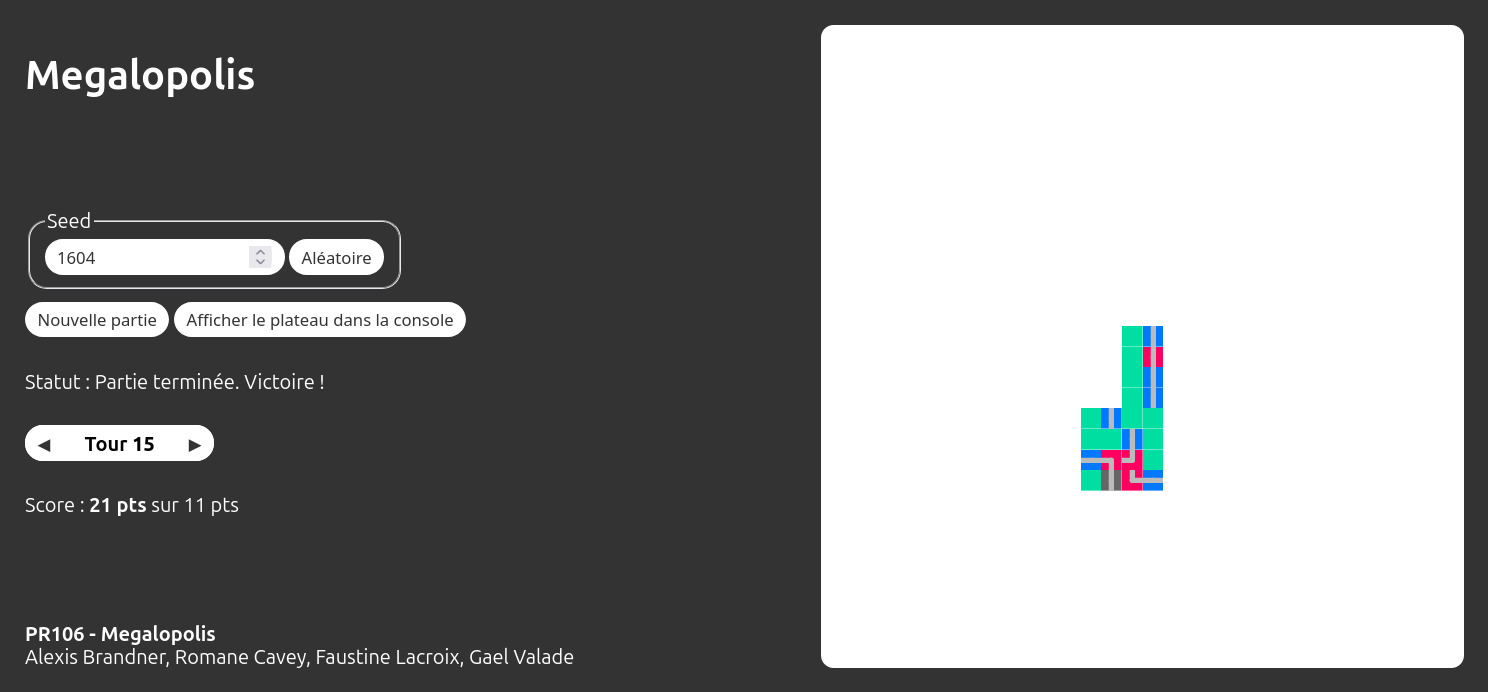
\includegraphics[width=0.75\linewidth]{images/Affichage/web-gui-v2.png}
    \caption{L'interface graphique}
    \label{fig:web_gui}
\end{figure}

Le plateau de jeu est représenté un élément \texttt{div}. Les tuiles sont découpées en quarts (comme dans le reste du jeu), qui sont placés dans le plateau. Le positionnement des quarts de tuiles sur le plateau se fait à l'aide d'une grille CSS et des propriétés \texttt{grid-column: x; grid-row: -y;} (l'axe des $y$ étant orienté vers le bas dans les grilles CSS).

Sur le plateau, chaque quart de tuile est représenté par un élément \texttt{svg} (dessin vectoriel). Ces dessins sont générés par le code, dessinant un rectangle pour la couleur de fond et deux lignes pour la route.

Le panneau de contrôle contient différents éléments~:
\begin{itemize}
    \item Un bouton permettant de lancer une partie
    \item Un bouton permettant d'avancer au tour suivant
    \item Un bouton permettant de retourner au tour précédent
    \item Un bouton permettant d'afficher la représentation textuelle du plateau dans la console du navigateur (utilisé pour le débugage)
    \item Un affichage de certaines informations utiles (n° du tour, score actuel, score requis pour gagner, etc.)
    \item Un champ permettant de spécifier une seed à utiliser
\end{itemize}

\subsubsection{Lien avec le reste du code — Interactivité}

Pour lier le reste du projet à notre interface graphique, on inclus dans le fichier \texttt{html/app.ts} (script associé à la page HTML, voir section~\ref{sec:parcel}) différents éléments provenant de nos autres fichiers de code. Afin de rendre l'exécution interactive, le code présent dans le fichier \texttt{src/main.ts} a été découpé 4 fonctions et copié dans un fichier \texttt{src/interactive.ts}. Le découpage suivant permet une exécution tour-par-tour de la partie, rendant l'affichage des premiers tours plus rapide~:

\begin{itemize}
    \item \texttt{initGame} : initialise une partie à partir d'une seed,
    \item \texttt{objScore} : calcule le score à atteindre pour remporter la partie,
    \item \texttt{playTurn} : joue une tour,
    \item \texttt{score} : calcule le score actuel.
\end{itemize}

Ces différentes fonctions sont appelées depuis \texttt{html/app.ts}, lorsque l'utilisateur appui sur certains boutons de la page (détection de l'évènement \texttt{click} avec la fonction \texttt{element.addEventListener}).

\subsubsection{Utilisation du bundler Parcel}

Parcel est un bundler permettant de livrer facilement une interface web. Parcel s'occupe de lancer localement un serveur web sur lequel va être hébergé une application. Cette application doit être fournie sous la forme suivante~:

\begin{itemize}
    \item Un document \texttt{index.html}, contenant la structure de la page web.
    \item Un script \texttt{app.ts}, qui est le script associé à la page. C'est ce script qui permettra de faire le lien entre le DOM (Document Object Model, qui contient les éléments HTML de notre page) et le code TypeScript que l'on a écrit pour l'application.
    \item Une feuille de styles \texttt{styles.css}, qui pourra contenir les différentes règles de mise en forme des éléments présents à l'écran.
\end{itemize}

% nécessite index.html, app.ts, et styles.css : compile les fichiers nécessaires & les distribue au client
% héberge localement

\label{sec:parcel}


%%% Boucle de jeu :
\section{Boucle de jeu}
Une boucle de jeu pour un langage de programmation pour qui la boucle n'est pas naturelle, cela peut paraître surprenant !

\subsection{Fonctionnement du jeu — Pureté}
Faire une boucle de jeu sans boucle a été l'un des points clés du projet. Pour réaliser la boucle de jeu on effectue un \texttt{reduce} sur les cartes de la pioche. La fonction passée en paramètre du \texttt{reduce } est la suivante: on cherche la position la plus avantageuse pour notre joueur (voir stratégie section \ref{subsec:Strategie} ) et on crée un nouveau plateau et de nouveaux graphes avec la tuile qui a été ajouté. L'accumulateur passé en paramètre est la liste \texttt{Map(board: aNewBoard, cGraph: aNewCGraph, rGraph: aNewRGraph)}, et est initialisé avec des plateaux et graphes vides. \\
Cela nous permet de garantir la pureté de notre boucle de jeu.


\subsection{Stratégie}
\label{subsec:Strategie}
Initialement, la pose des tuiles sur le plateau se réalisait de manière aléatoire, ce qui aboutissait le plus souvent à une défaite, avec un score fréquemment négatif. Pour remédier à ce problème, nous avons décider de mettre en place une stratégie.

Afin de ne jouer que les meilleurs coups pour chaque tuile, on teste toutes les positions possibles en calculant le score, en considérant la tuile à cette position donnée. On ne garde que le meilleur coup (s'il y en a plusieurs, on ne garde que le premier). Pour augmenter notre score, nous avons augmenté notre nombre de coups possibles~: grâce à la fonction \texttt{flip\_tile}, nous prenons aussi en compte la rotation de la tuile. Ainsi si le fait de tourner la tuile nous est avantageux, c'est ce qu'on fait sinon on garde la tuile telle quel. 

\subsection{Améliorations possibles}
L'un des défauts de notre stratégie est qu'elle privilégie le maximum local et pas forcément le maximum global.
Pour encore optimiser la stratégie, on pourrait faire du deep learning ou faire le calcul de score sur les coups suivants. 
La contrainte de temps ne nous a pas permis d'approfondir ces pistes.


%%% Tests :
\section{Tests}
Les tests sont incontournables, ils permettent de verifier que les fonctions respectent leur signature.

\subsection{Utilisation de Jest}
L'un des objectifs de ce projet était de découvrir et prendre en main le framework Jest. Ce dernier est un environnement de travail pour réaliser des tests sous JavaScript (et compatible avec TypeScript). On a de nombreuses fonctions à disposition pour faire les tests notamment \texttt{test}, \texttt{expect} et \texttt{toBe}. Jest offre un affiche clair des tests qui passent ou pas, ce qui permet une correction rapide.

\subsection{Les fonctions et leur tests}
Les personnes faisaient les tests des fonctions qu'ils programmaient dans un soucis de performances. En effet une personne qui implémente un fonction connaît déjà les entrées et sorties de celle-ci donc peut faire les tests plus rapidement. Cependant nous avons remarqué que des cas limites sont oubliés ou pire encore que les tests sont faux car implémentés d'une façon trop proche à celle de la fonction.

Prenons l'exemple illustré par la figure~\ref{fig:ex_autre_tests}. Celui qui a codé la fonction \texttt{flip\_tile} (qui permet de tourner la tuile) a permuté les routes sans les tourner c'est-à-dire juste comme les quartiers. Les tests réalisés vérifiaient juste que les routes étaient permutées mais pas qu'elles étaient encore correctement connectées les une au autre. Donc les tests validaient une fonction incorrecte. Ainsi il vaut mieux qu'une autre personne fasse les tests même si c'est plus long.

\begin{figure}[H]
    \centering
    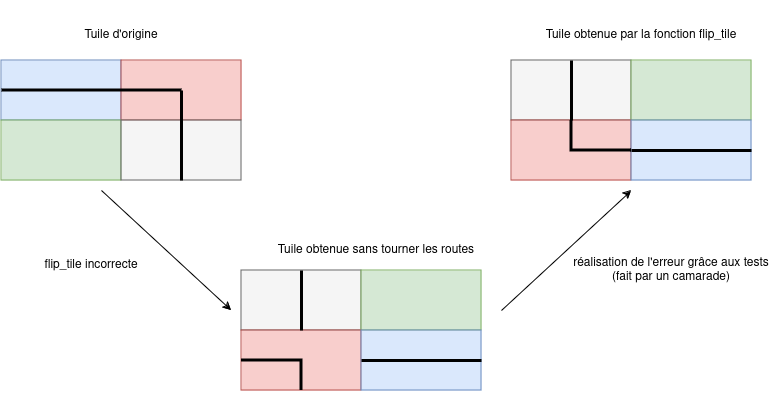
\includegraphics[width=0.8\linewidth]{images/tests/autre_fait_test.png}
    \caption{Problème du test fait par la personnes qui a codé la fonction}
    \label{fig:ex_autre_tests}
\end{figure}

Pour tester certaines fonctions, notamment celle dans \texttt{src/objectives.ts}, nous avions besoin d'avoir une partie reproductible, dont le résultat est attendu. Pour cela, nous avons utilisé le concept de \texttt{seed}~: pour une \texttt{seed} donnée, la partie jouée est la même. C'est l'identifiant d'une partie.

\subsection{Couverture}

La couverture du code est une métrique qui peut vous permettre de comprendre la part testée de nos sources, elle permet une meilleur fiabilité de celles-ci, en effet un code testé à 80\% donnera plus confiance en son utilisation qu'un code pas testé du tout. Afin de savoir le pourcentage de fonctions que nous testons il nous faut utiliser l'option \texttt{--coverage} sur la commande \texttt{npx jest}, la figure~\ref{fig:couverture} montre la couverture de nos tests.
Cette figure nous montre uniquement ce que nous testons mais pas si nos tests sont pertinents. Cependant comme nous pouvons le voir nos sources sont testés à 92\% ce qui assure au moins une certaine stabilité et fiabilité du code.

\begin{figure}[H]
    \centering
    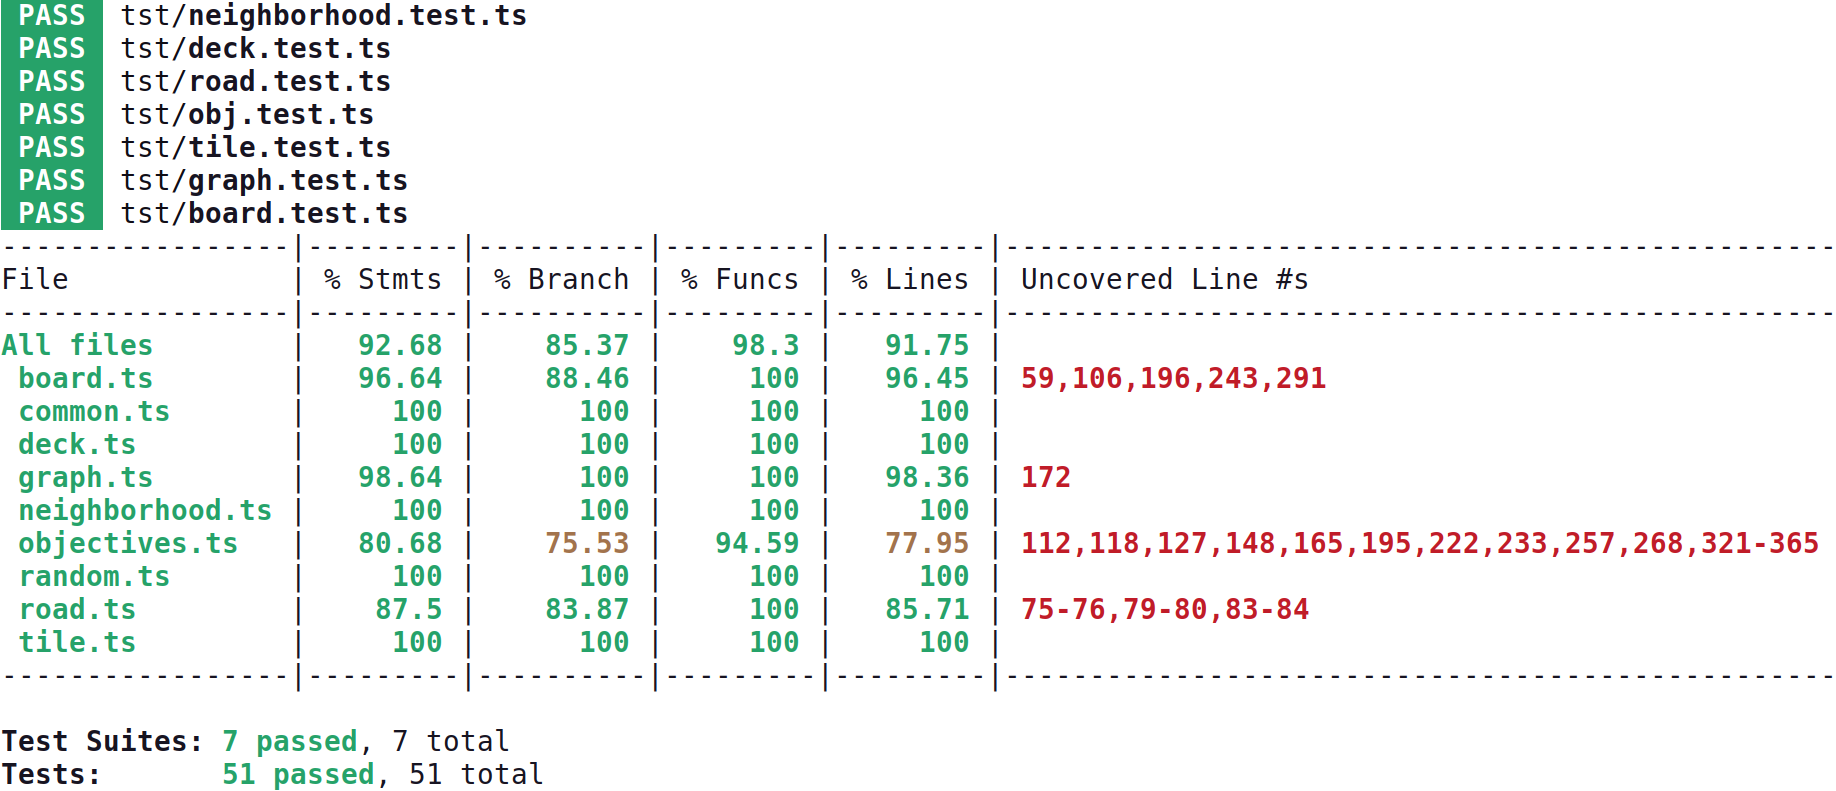
\includegraphics[width=0.9\linewidth]{images/tests/couverture_test.png}
    \caption{Couverture de nos tests}
    \label{fig:couverture}
\end{figure}


%%% Dificultés :
\section{Difficultés}

Lors de ce projet nous avons rencontré des difficultés qui nous ont posés problèmes, il nous semble important d'en parlé car c'est des problèmes qu'on apprend le plus. Par ailleurs, pour la plupart d'entre nous, c'était notre premier projet en ts.

\subsection{Problème de pureté}

La programmation fonctionnelle repose en partie sur la création de nouvelles instances à chaque appel de fonction. Donc en théorie nous avions besoin que du mot clé \texttt{const} pour déclarer des variables constantes et non de \texttt{let}. Cependant nous n'avons pas toujours réussi à appliquer cela par exemple dans le fichier \texttt{src/graph.ts}, la fonction \texttt{isCycle} utilise une boucle \texttt{while} (l'implémentation étant plus simple comme ça, bien qu'aussi réalisable avec une fonction récursive) et donc nécessite l'utilisation de variables déclarées avec le mot-clé \texttt{let}, celles-ci devant être modifiables après déclaration.

\subsection{Envie de faire des boucles}
Par habitude, avec les langages C ou Python, nous avons l'automatisme de faire des boucles, ce qui s'est avéré plus complexe en programmation fonctionnelle. Pour la boucle de jeu notamment, nous avons dû utiliser un \texttt{reduce}, sur les cartes du \texttt{Deck}. Les \texttt{reduce} et \texttt{map} ont remplacé les boucles classiques, puisqu'ils permettent d'itérer sur les éléments d'une liste. Dans certains cas, nous avons passé en paramètre un compteur $i$ , qu'on décrémente ou incrémente à chaque appel de la fonction, telle que la condition d'arrêt dépend de la valeur de $i$. 





%%% Répartition du travail
\section{Répartition du travail}

Pour trois d'entre-nous c'était la première fois que nous faisions un projet par groupe de quatre, cependant la division du travail s'est fait naturellement. Nous avons commencé par travailler en peer-programming afin d'être sur de tous partir sur les mêmes bases puis nous nous sommes chacun répartis les tâches et si nécessaire se remettre en peer-programming pour résoudre des problèmes plus complexe.

%pose syndical, goûter.
\subsection{Peer-programming}
Le choix du Peer-programming a été fait afin de confronter nos idées et ainsi trouver la meilleure implémentation possible. Le projet nous laissant libre sur certaines implémentations, il fallait que chaque membre du groupe puisse participer leurs conceptions. Par ailleurs d'après le cours PG106, cette stratégie permet de limiter les erreurs dans le code, étant donné qu'il y a au moins 2 relecteurs pour un même code. Cela nous a permis d'appréhender une nouvelle technique de programmation.




%% Conclusion :
\section{Conclusion}

A travers ce projet nous avons implémenté le jeu Megalopolis. Ce projet nous a permis de mieux prendre en main le langage TypeScript et surtout nous a permis d'appliquer les connaissances acquises en cours de programmation fonctionnelle.

\subsection{Ressenti sur le projet}

Nous avons trouvé ce projet encore plus intéressant et plus riche que celui du semestre 5. Se forcer à utiliser ces techniques de programmation particulières nous a montré que dans certains cas les fonctions pouvaient être codées beaucoup plus naturellement et facilement. Notamment l'utilisation des \texttt{map} et des \texttt{reduce} s'est révélée naturelle.

De plus ce sujet de TS étant très libre, nous avons pu discuter sur la façon de faire, échanger nos points de vu et finir par poser notre propre implémentation en connaissance de cause. Ce qui nous a vraiment plu car on avait une compréhension fine du projet.

\subsection{Retour sur les attendus}

A travers ce projet, nous avons appliqué ce que nous avons appris en cours de programmation fonctionnelle. Voici notamment les principaux points~: l'utilisation des typages, l'utilisation de la librairie \texttt{Immutable.js}, la pris en main de \texttt{jest}, de \texttt{ESLint} et de \texttt{Parcel} et comme dit précédemment la prise en main des fonctions récursives communes tel que \texttt{map} et \texttt{reduce}. Finalement c'est avec ces attendus que nous avons réussi à implémenter le jeu Megalopolis.




\end{document}
